% https://books.google.com/books?id=QQJODwAAQBAJ&pg=PA101&lpg=PA101&dq=%E2%80%9Cthe+secret+to+successful+hiring+is+this:+look+for+the+people+who+want+to+change+the+world.%E2%80%9D&source=bl&ots=D6l8JXfB20&sig=ACfU3U0x1X9Gh8k6MlNV0BqhBa_73Q0yfQ&hl=en&sa=X&ved=2ahUKEwj48pqg_oHgAhVohuAKHYlJAsc4ChDoATAAegQIChAB#v=onepage&q=%E2%80%9Cthe%20secret%20to%20successful%20hiring%20is%20this%3A%20look%20for%20the%20people%20who%20want%20to%20change%20the%20world.%E2%80%9D&f=false
% "The secret to successful hiring is this: look for the people who want to change the world.".  Marc Benioff.

NumPy is both a cause and an effect of a striking shift in the nature of
scientific computing.  The traditional model of scientific software has been of
the user as {\it consumer}.  Writing software is a task for specialists and
professionals, supported by income from selling the software to scientists to
use.  The new model is of the user as {\it owner}.  The Python language, with
the NumPy library, provides a framework that scientists can consume, but has
also been successful in encouraging scientists to develop as programmers, and
to write code for the library, and the system of packages around it.  This has
fostered a new culture of contribution and collaboration in scientific
computing that resulted in a virtuous cycle of increasing use, and increasing
development.

This cycle is one of several explanations for the astonishing growth of NumPy
in scientific computing.

\section*{History}

The first incarnation of NumPy was a package called Numeric, written in 1995
by Jim Hugunin, then completing his master's thesis at MIT on
superconductor-semiconductor junctions.  Hugunin based his package on previous
work by Jim Fulton, then working at the US Geological Survey, and acknowledges
many others in his initial report of the package \cite{Hugunin-whitepaper}.
Numeric provided an array object in Python, written in C, and linking to
standard fast implementations of linear algebra.

As Hugunin points out, at the time he wrote Numeric, commercial languages for
interactive computing with numerical arrays were already well-established,
including Matlab and IDL.  At the time, it must have seemed a safe bet that
Numeric would not succeed in this market.  The commercial languages were
developed and maintained by large numbers of full-time professional programmers
and supported by formal quality assurance, release managers and writers of
scientific documentation.  In contrast, Numeric, and later, NumPy, would
continue to be developed almost entirely by scientists, including graduate
students and faculty, without specific funding, and often to the detriment of
the scientists' careers.

Table X1 about here: backgrounds of initial designers (mainly math, physics).

Table X2 about here: backgrounds of major committers (mainly math, physics).

Around 1998, the Space Telescope Science Institute (STScI) software group began
to use Python heavily, and, around 2000, wrote a re-implementation of much of
Numeric, called NumArray, to support their need to work on large memory-mapped
arrays, and arrays of mixed data type records \cite{STScI-slither}.  This
briefly caused the Numeric and NumArray communities to diverge, until 2005,
when Travis Oliphant embarked upon a major rewrite that aimed to be a ``best of
both worlds'' unification of Numeric and NumArray \cite{oliphant2006guide}.
This merger resulted in NumPy.  At the time, Oliphant was an assistant
professor of Electrical and Computer Engineering at Brigham Young University.

Over the next 10 years, NumPy attracted a relatively large pool of scientist
developers.  To benefit from these
user-developers, the project developed an increasingly strong culture of using
software-engineering practice to improve collaboration and reduce error
\cite{millman2014developing}. The NumPy team was early in adopting distributed
revision control and code review to improved collaboration on code, and
continuous testing so we run a large battery automated tests for every proposed
change in NumPy. At first, NumPy had rather sparse documentation, but the project
developed a new standard for ``docstrings''---text describing each NumPy
function---and used this standard to write comprehensive high-quality
documentation, integrated with the source code. The NumPy documentation format
quickly became a standard for the larger Python community.

\begin{figure}
    \centering
    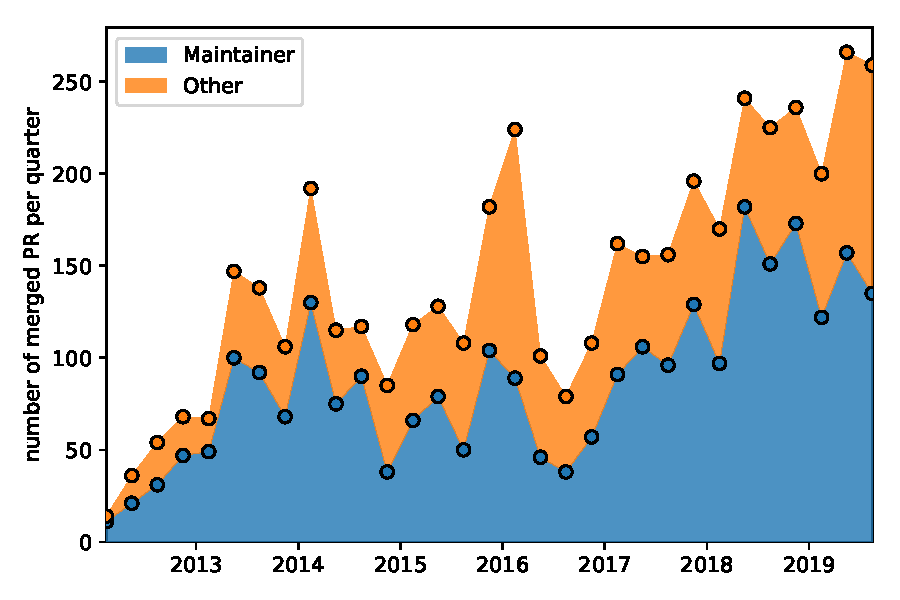
\includegraphics[width=0.9\linewidth]{scripts/PRs-using-CURRENT_MAINTAINERS.pdf}
    \caption{Number of pull requests merged into the NumPy master branch for each
        quarter since 2012. The total number of PRs is indicated with the
        lower blue area showing the portion contributed by current or previous
        maintainers.}\label{fig:prs-over-time}
\end{figure}

NumPy is currently maintained by a group of 23 contributors with commit rights
to the NumPy code base. Out of these, 17 maintainers were active in
2019, 4 of whom were paid to work on the project full-time.
Additionally, there are a few long term developers who contributed and maintain
specific parts of NumPy, but are not officially maintainers.
At a release cycle of about every half year, the five recent releases in the years
2018 and 2019 have averaged about 450~pull requests~(PRs) each,\footnote{
    Note that before mid 2011, NumPy development did not happen on \url{github.com}.
    All data provided here is based on the development which happened through GitHub
    pull requests. In some cases contributions by maintainers may not be categorized as such.}
% Since 1.14.0 (based on changelog): 381 + 438 + 490 + 531 + 402; last is preliminary
with each release attracting more than a hundred new contributors.
Figure~\ref{fig:prs-over-time} shows the number of PRs merged into the NumPy
master branch.
Although the number of PRs being merged fluctuates,
the plot indicates an increased number of contributions over the past
years.

\section*{Enabling factors}

The creation of NumPy spurred renewed development in the larger scientific
Python ecosystem and heralded the current era of wide-spread use of Python for
scientific computing.
As we implied above, there were several factors that allowed this rapid growth
and successful development.

Hugunin identified the first factor in his initial description of the Numeric
package \cite{Hugunin-whitepaper}.  Numerical computing is usually one
component of a larger programming task.  Therefore:

\begin{quote}
    Rather than trying to retrofit an existing numerical language to support
    the wealth of features found in a powerful, modern, general-purpose
    programming language, it makes much more sense to attack the problem from
    the other direction and add the features of a powerful numerical
    programming language to Python.
\end{quote}

Python is already a good choice for many standard programming tasks such as
cleaning data, interacting with web resources and parsing text.  It has a wide
range of libraries for many different tasks. Adding fast array operations and
linear algebra allows the scientist to do all their work with within the same
language---and one that has the advantage of being famously easy to learn and
teach.

The second factor flows from Python's nature as an open-source language,
embedded within the open-source community.  Python attracts developers who like
to build and contribute.  As a result, NumPy has always been a library that was
developed by scientists in order to do their work.  Commercial specialist
numerical languages can encourage consumer-users, who pick up a tool and use
it, but do not expect to contribute to development.  In contrast, NumPy often
attracts user-developers, who want to work with NumPy, and are prepared to fix
and extend the library as they work. User-developers have been the fundamental
force in developing NumPy, and shaping it into a library that has been refined
in the furnace of practical scientific work.

The third factor is much like the second: a culture in Python that concentrates
on high quality of code and distribution. Because Python is open-source, it has
a strong culture of contribution, and therefore, of using tools and process to
improve collaborative software development, such as distributed version
control, code review, and automated testing.  These have allowed the project to
scale safely as it attracted more users and developers, even though these
developers rarely came to the project with training in software engineering.

Lastly, we believe NumPy has benefited greatly from a well-chosen application
programming interface (API).  Scientific and numerical programming needs to be
fast, and scale to very large datasets.  The NumPy API defines a simple wrapper
for data in memory so it can be represented as a one- or multi-dimensional
array.  The simplicity of this wrapper has made it very successful as a
standard way of representing arrays in memory, and has made it relatively easy
for other libraries to develop fast and memory-efficient compiled code, usually
in C or Fortran, that can manipulate these arrays and pass them back to Python.
This has been a large factor in the growth of numerical computing libraries
around NumPy and Python.


\section*{NumPy arrays}


With its first stable release in October 2006, NumPy unified
the scientific Python community and now underpins almost every library
that does numerical computation, including SciPy\cite{virtanen2019scipy},
pandas\cite{mckinney-proc-scipy-2010}, scikit-learn\cite{pedregosa2011scikit},
and scikit-image\cite{vanderwalt2014scikit}.
NumPy consists of the \code{ndarray}-object along with utility functions that
operate on it.
Because of its inherent simplicity---being a pointer to memory with some
associated meta-data about shape, data-type, and so forth---the NumPy array is
the {\it de facto} exchange format for array data in Python.
The library has such widespread adoption that not only the array object but also its
{\it Application Programming Interface} (API) has become ubiquitous as
a language for tensor computation---witnessed by its use in popular
deep learning libraries such as PyTorch\cite{pytorch}.

The \code{ndarray} data structure stores regularly spaced elements of a single
data type in a contiguous block of memory; along with meta-data such as shape,
it allows for the efficient representation of $n$-dimensional arrays \cite{vanderwalt2011numpy}.
The need for such a data structure arises often in science.
For instance, they may store measurements from an experiment or simulation
at discrete time points.

Data analysis frequently involves operations $(+, -, \times, /, \log, \sin, \dots)$ on
the individual measurements.
In programming languages such as C or Java, this would involve looping over
every element to perform these operations.
Array computations generalize these element-wise operations on scalars to
vectors (1-d arrays), matrices (2-d arrays), and higher dimensional arrays (n-d
arrays).
For instance, if \code{x} is an \code{ndarray}, then \code{2 * x} produces
an \code{ndarray} whose values are twice those in \code{x}.
Similarly, if \code{x} and \code{y} have the same shape, then
\code{x * y} produces an \code{ndarray} whose values are the products of
the corresponding entries of \code{x} and \code{y}.
These \emph{vectorized} operations often produce one-liners that would be tens
or hundreds of lines of code in languages such as C.

Element-wise operations are not always desired.
Suppose the matrix \code{A} is a 2-d array and the vector \code{x} is 1-d array.
Then \code{A @ x} computes the matrix-vector product $Ax$ and
\code{x @ A} computes the vector-matrix product $x^\top A$.
This matrix multiplication operation extends to higher-dimensions by
treating the array as a stack of matrices.

NumPy also provides a large collection of functions for array manipulation
including functions for: creating, reshaping, concatenating, and padding arrays;
searching, sorting and counting data
in arrays; computing elementary statistics, such as the mean, median,
variance, and standard deviation; file I/O; and more.
It also provides extensive support for generating pseudorandom numbers
as well as an assortment of probability distributions.
For historical reasons, NumPy also includes basic functionality for
linear algebra, fast Fourier transforms and windowing,
and polynomial fitting.
We will continue supporting these, but we will not expand beyond them.

\section*{Hybrid development}

For many years, NumPy had no dedicated funding, and development time
was mostly contributed freely by students and researchers in their
spare time.  In-person meetings were sponsored off of individual's
research grants, and while industry sponsored contributions were made,
notably those by Mark Wiebe when he was sponsored by Travis Oliphant
at Continuum Analytics, the package's rapid adoption in scientific
computing took place without external investment.

% BIDS -- UCB
% https://www.moore.org/grant-detail?grantId=GBMF5447
% $645,020 in 2016
% https://sloan.org/grant-detail/8222
% $659,359 in 2017
% https://bids.berkeley.edu/news/bids-receives-sloan-foundation-grant-contribute-numpy-development
% http://doi.org/10.5281/zenodo.3585761
% http://doi.org/10.5281/zenodo.3585767
In 2017, NumPy received its first large grants totaling 1.3M USD from the
Gordon \& Betty Moore and the Alfred P. Sloan foundations.
These two grants focus on addressing the technical debt accrued over the years and
on setting in place standards and architecture to encourage more sustainable development.
% CZI -- NumFOCUS/QuanSight
% https://chanzuckerberg.com/eoss/proposals/strengthening-numpys-foundations-growing-beyond-code/
% NumPy and OpenBLAS received $195,000 in 2019
% https://labs.quansight.org/blog/2019/11/numpy-openblas-CZI-grant/
NumPy received a third grant for 195K USD from the Chan Zuckerberg
Initiative at the end of 2019.
This grant focuses on better serving NumPy's large number of beginning
to intermediate level users and on growing the community of NumPy
contributors.
Finally, the project receives around 10K USD annually from Tidelift, which is
typically used to fund documentation writers and website developers.

The first activities organized for the new grants were a development planning
sprint, a weekly community call, and a meeting to write a draft roadmap.
Since the roadmap was meant to represent community consensus on future
development, it was presented for comment at the annual SciPy
conference during a so-called ``Birds of a Feather'' session, attended
by more than 100 people.  One additional meeting was held to discuss
specific enhancements, such as the development of a new data-type
system.  The final roadmap was vetted by the community via online
discussion before being accepted.

With the recent infusion of funding and a clear process for coordinating with
the developer community, we have been able to tackle a number of important
large scale changes.
We highlight two of those below.

\section*{Array function protocol}

A vast number of projects are built on NumPy;
these projects are consumers of the NumPy API.
Over the last several years, a growing number of projects are providers of
a \emph{NumPy-like API} and array objects targeting audiences with specialized
needs beyond NumPy's capabilities.
For example, the NumPy API is implemented by several popular tensor computation
libraries including CuPy\footnote{\url{https://cupy.chainer.org/}},
Jax\footnote{\url{https://jax.readthedocs.io/en/latest/jax.numpy.html}},
PyTorch\footnote{\url{https://pytorch.org/tutorials/beginner/blitz/tensor\_tutorial.html}}, and
and Apache MXNet\footnote{\url{https://mxnet.incubator.apache.org/api/python/docs/api/ndarray/index.html}}.
It is also implemented in packages that support sparse arrays
such as \code{scipy.sparse} and \code{pydata.sparse}.
Another notable example is Dask, a library for parallel computing in
Python.  Dask adopts the NumPy API and therefore presents a familiar
interface to existing NumPy users, while adding powerful abilities to
parallelize and distribute tasks.

The multitude of specialized projects creates the difficulty that consumers
of these NumPy-like APIs write code specific to a single project and do not support
all of the above array providers.
This is a burden for users relying on the specialized array-like, since
a tool they need may not work for them.
It also creates new challenges for end-users who need to transition
from NumPy to a more specialized array.
The growing multitude of specialized projects with NumPy-like APIs threatened
to again fracture the scientific Python community.

To address these issues NumPy has the goal of providing the fundamental
API for \emph{interoperability} between the various NumPy-like APIs.
An earlier step in this direction was the implementation of the
\code{\_\_array\_ufunc\_\_} protocol in NumPy 1.13, which enabled interoperability
for most mathematical functions.\cite{NEP13}
In 2019 this was expanded more generally with the inclusion of the
\code{\_\_array\_function\_\_} protocol into NumPy~1.17.
These two protocols allows providers of array-like APIs to be interoperable
with the NumPy API: their arrays work correctly with almost all NumPy functions.\cite{NEP18}
For the users relying on specialized array projects it means that even though
much code is written specifically for NumPy arrays and uses the NumPy API as
\code{import numpy as np}, it can nevertheless work for them.  For
example, here is how a CuPy GPU array can be passed through NumPy for
processing, with all operations being dispatched back to CuPy:

\begin{lstlisting}
import numpy as np
import cupy as cp

x_gpu = cp.array([1, 2, 3])
y = np.sum(x_gpu)  # Returns a GPU array
\end{lstlisting}

\section*{Random}

The NumPy random module provides pseudorandom numbers from a wide range of
distributions. In legacy versions of NumPy, simulated random values are produced
by a \code{RandomState} object that: handles seeding and state initialization;
wraps the core pseudorandom number generator based on a 32-bit implementation of
MT19937; interfaces with the underlying code that transforms random bits into
deviates from other distributions; and supplies a singleton instance exposed in
the root of the random module.

The \code{RandomState} object makes a compatibility guarantee so that a fixed
seed and sequence of function calls produce the same set of values. This
guarantee has slowed progress since improving the underlying code requires
extending the API with additional keyword arguments. This guarantee continues to
apply to \code{RandomState}. 

NumPy 1.17 introduced a new API for generating random numbers that use a more
flexible structure that can be extended by libraries or end-users. The new API
is built using components that separate the steps required to generate random
variates. Pseudorandom bits are generated by a bit generator. These bits are
then transformed into variates from complex distributions by a generator.
Finally, seeding is handled by an object that produces sequences of high-quality
initial values.

Bit generators are simple classes that manage the state of an underlying
pseudorandom number generator. NumPy ships with four bit generators. The default
bit generator is a 64-bit implementation of the Permuted Congruential Generator
\cite{pcg64} (\code{PCG64}). The three other bit generators are a 64-bit version
of the Philox generator\cite{random123} (\code{Philox}), Chris Doty-Humphrey's
Small Fast Chaotic generator\cite{practrand} (\code{SFC64}), and the 32-bit
Mersenne Twister\cite{mt19937} (\code{MT19937}) which has been used in older
versions of NumPy.\footnote{The
\href{https://github.com/bashtage/randomgen}{randomgen project} supplies a wide
range of alternative bit generators such as a cryptographic counter-based
generators (\code{AESCtr}) and generators that expose hardware random number
generators (\code{RDRAND})\cite{randomgen}.} Bit generators export a capsule
containing pointers to functions that produce 64 bits, 32 bits, or a random
double. They also expose CFFI and ctypes interfaces to the same three functions.

The \code{Generator} consumes one of the bit generators and produces variates
from complicated distributions. Many improved methods for generating random
variates from common distributions were implemented, including the Ziggurat
method for normal, exponential and gamma variates\cite{ziggurat}, and Lemire's
method for bounded random integer generation\cite{lemire}. The \code{Generator}
is more similar to the legacy \code{RandomState}, and its API is substantially
the same. The key differences all relate to state management, which has been
delegated to the bit generator. The \code{Generator} does not make the same
stream guarantee as the \code{RandomState} object, and so variates may differ
across versions as improved generation algorithms are
introduced.\footnote{Despite the removal of the compatibility guarantee, simple
reproducibility across versions is encouraged, and minor changes that do not
produce meaningful performance gains or fix underlying bug are not generally
adopted.}

Finally, a \code{SeedSequence} is used to initialize a bit generator. The seed
sequence can be initialized with no arguments, in which case it reads entropy
from a system-dependent provider, or with a user-provided seed. The seed
sequence then transforms the initial set of entropy into a sequence of
high-quality pseudorandom integers, which can be used to initialize multiple bit
generators deterministically. A key design goal of a seed sequence was to be
splittable in the sense that a seed sequence can be used to produce child
sequences that are distinct from their parents or other ancestors. This
capability allows a seed sequence to be used in large distributed applications
where the number of workers required is not known. The sequences generated from
the same initial entropy and the same splits are fully deterministic to ensure
reproducibility.

The three components are combined to construct a complete random number
generator.

\begin{lstlisting}
from numpy.random import (
    Generator,
    PCG64,
    SeedSequence,
)

seq = SeedSequence(1030424547444117993331016959)
pcg = PCG64(seq)
gen = Generator(pcg)
\end{lstlisting}

\noindent This approach retains access to the seed sequence which can then be
used to spawn additional generators.

\begin{lstlisting}
children = seq.spawn(2)
gen_0 = Generator(PCG64(children[0]))
gen_1 = Generator(PCG64(children[1]))
\end{lstlisting}

\noindent While this approach retains complete flexibility, the method
\code{np.random.default\_rng} can be used to instantiate a \code{Generator} when
reproducibility is not needed.

The final goal of the new API is to improve extensibility. \code{RandomState} is
a monolithic object that obscures all of the underlying state and functions. The
component architecture is one part of the extensibility improvements. The
underlying functions (written in C) which transform the output of a bit
generator to other distributions are available for use in CFFI. This allows the
same code to be run in both NumPy and dependent that can consume CFFI, e.g.,
Numba. Both the bit generators and the low-level functions can also be used in C
or Cython code.\footnote{As of 1.18.0, this scenario requires access to the
NumPy source. Alternative approaches that avoid this extra step are being
explored.} 

\section*{Discussion}

% 1st grant done, technical cleanup finished except dtypes
% 2nd grant starting, community growth and new user focus

Most of the technical work for the Moore and Sloan grant is now complete.
The main remaining item is an overhaul of the data type system, which
we are currently working on.
The meaning of each element within a NumPy array is described by its
datatype (dtype). NumPy arrays can hold all common numerical
datatypes, strings, datetimes, and generic Python objects, each of
which is identified by a dtype.
%We are busy overhauling the datatype
%system to make it behave consistently and to simplify the creation of
%custom dtypes, both in C and in Python [XXX Cite the NEP here, instead
%of \href{https://github.com/numpy/numpy/pull/14422}{draft of DTypes NEP}].
While numerical dtypes make the foundation for most users,
there are a multitude of use cases which cannot prosper due to current
limitations, such as physical units\cite{astropy,Goldbaum2018,pint},
% pyadolc may be a bit too small a project, so may want to remove/replace with an other example.
geometrical objects\cite{pygeos}, and automatic
differentiation\cite{pyadolc}.
%Projects addressing these exist, each struggles with current
%limitations.  % TODO: I may need citations, we could link github issues.
The proposed overhaul of the datatype system will make it behave consistently and
to simplify the creation of custom dtypes, both in C and in Python

%% While it is currently possible to define custom dtypes within NumPy, many of the
%% use cases above cannot be solved using this system.
%% This is evidenced also by code within NumPy which would require changes
%% in many places to add such dtypes, even when adding them within NumPy itself.
%% The new implementation will be simpler and more cleanly implemented in
%% this regard.
%% Custom dtypes and the basic dtypes included within NumPy will be implemented
%% and behave identically as much as possible.
%% At the same time redesigning the API will make NumPy dtypes more flexible to grow
%% to future needs should they arise.

%% As a further step, to make dtypes more accessible and allow a faster adoption of
%% custom dtypes within the community, we plan to create a Python API to
%% define such custom dtypes.

Having made progress on addressing technical debt accrued over two decades of
development and modernizing the code to handle new use cases, the project
is ready to grow its community of contributors and to better address the needs
of an ever-growing number of new users.  This is the main focus of the
forthcoming CZI grant.

[... CZI grant ...]

[... welcome new users ...]

% technical focus
% improve various aspects of NumPy, including easier construction of custom data types (e.g., missing values, physical units, times & dates) and better integration with arrays customized for specialized domains (e.g., SciPy's sparse arrays, pandas' DataFrames, and xarray's labeled arrays). 
% technical work, and it increased the velocity of the projects by ~25-30%, and in addition it enabled integrating some larger changes, like the numpy.random redesign.


% \subsubsection*{Future Development}

% Dtypes

% outline plan for the CZI grant and an invitation to new contributors

%\subsection*{Website}
